\documentclass[11pt,a4paper]{article}
\usepackage[T1]{fontenc}
\usepackage[utf8]{inputenc}
\usepackage{lmodern}
\usepackage[margin=25mm]{geometry}
\usepackage{amsmath,amssymb,amsthm,booktabs,longtable,tabularx,array}
\usepackage{graphicx,microtype,xurl}
\usepackage[round,authoryear]{natbib}
\usepackage[hidelinks]{hyperref}
\usepackage{caption,enumitem}
\captionsetup{font=small,labelfont=bf}
\setlength{\parskip}{3pt}
\setlength{\parindent}{1em}
\setlength{\emergencystretch}{3em}
\renewcommand{\arraystretch}{1.14}
\newtheorem{proposition}{Proposition}
\newcommand{\E}{\mathbb{E}}
\newcommand{\R}{\mathbb{R}}
\newcommand{\ind}{\mathbf{1}}
\newcommand{\ResultPOneMviGdp}{0.00}
\newcommand{\ResultPOneTaxGdp}{17.77}
\newcommand{\ResultPOneGiniWealth}{0.788}
\newcommand{\ResultPOneUsownershipShare}{0.00}
\newcommand{\ResultPOneMedianIncome}{1.420}
\newcommand{\ResultPOneMaxInflation}{2.04}
\newcommand{\ResultPTwoMviGdp}{19.03}
\newcommand{\ResultPTwoTaxGdp}{37.04}
\newcommand{\ResultPTwoGiniWealth}{0.754}
\newcommand{\ResultPTwoUsownershipShare}{0.00}
\newcommand{\ResultPTwoMedianIncome}{2.183}
\newcommand{\ResultPTwoMaxInflation}{2.17}
\newcommand{\ResultPFiveMviGdp}{10.57}
\newcommand{\ResultPFiveTaxGdp}{28.53}
\newcommand{\ResultPFiveGiniWealth}{0.583}
\newcommand{\ResultPFiveUsownershipShare}{29.67}
\newcommand{\ResultPFiveMedianIncome}{2.392}
\newcommand{\ResultPFiveMaxInflation}{2.12}
\newcommand{\ResultPSixMviGdp}{10.16}
\newcommand{\ResultPSixTaxGdp}{27.13}
\newcommand{\ResultPSixGiniWealth}{0.584}
\newcommand{\ResultPSixUsownershipShare}{29.67}
\newcommand{\ResultPSixMedianIncome}{2.415}
\newcommand{\ResultPSixMaxInflation}{2.13}
\newcommand{\ResultPSevenMviGdp}{5.96}
\newcommand{\ResultPSevenTaxGdp}{23.91}
\newcommand{\ResultPSevenGiniWealth}{0.560}
\newcommand{\ResultPSevenUsownershipShare}{29.67}
\newcommand{\ResultPSevenMedianIncome}{2.293}
\newcommand{\ResultPSevenMaxInflation}{2.12}
\newcommand{\SensitivityCount}{128}
\newcommand{\SensitivitySunsets}{6}
\newcommand{\SensitivityPriceBand}{128}
\newcommand{\MaxAccountingError}{6.19e-16}

\usepackage{xr}
\externaldocument[M-]{main}
\renewcommand{\thesection}{S\arabic{section}}
\renewcommand{\thetable}{S\arabic{table}}
\renewcommand{\thefigure}{S\arabic{figure}}
\title{Online Supplement\\\large Bridging the AI Ownership Transition: Usownership, Programmable Money and the Limits of Seigniorage}
\author{}\date{9 September 2026}
\begin{document}\maketitle
This supplement provides terminological provenance, the Internet-of-Value implementation boundary, complete laboratory equations, scenario definitions, additional paths and reproduction checks. It distinguishes inherited experiments from the new comparative extension. Values are synthetic model outputs, not empirical forecasts. The main paper provides the comparative propositions and institutional interpretation.
\section{Terminological provenance and bounded prior-use search}
The exploratory notebooks used the working expression ``useownership''. The present revision adopts \emph{usownership} as the noun for the generalised institution, but the associated \emph{Usowner} concept is not being backdated to 2026. ERC-4950, created on 28 March 2022 by V\'ictor Mu\~noz, Josep Lluis de la Rosa and Easy Innova, explicitly lists ``Usowners'' among its applications and glosses them as users who consume an NFT and become partial owners \citep{erc4950}. The same proposal implements a pair of entangled ERC-721 tokens that can jointly operate a smart-contract wallet. Its current status is \emph{Stagnant}; the manuscript therefore calls it a standards-track ERC proposal or technical precursor, not an adopted Ethereum standard.

The present noun is constructed from the same semantic transition: \emph{user} $\rightarrow$ \emph{Usowner} $\rightarrow$ \emph{usownership}, where \emph{-ship} denotes the durable ownership relation. What is new in the present paper is the generalisation from an NFT-oriented partial-owner use case to a recurring corporate mechanism with graded contribution, dilution accounting and macroeconomic transition dynamics. The 2022 ERC does not contain the contribution-score equation, automation-linked issuance schedule, matched fiscal benchmark or monetary-financing model used here. This distinction is important because it lets the paper claim continuity without claiming novelty for its own precursor.

The prior-use check was designed to avoid an unsupported lexical claim rather than to establish trademark clearance. On 9 September 2026 exact-string searches were run for ``usownership'' and variants combined with \emph{ownership}, \emph{user ownership}, \emph{platform}, \emph{cooperative}, \emph{patent}, \emph{trademark}, \emph{book} and \emph{dictionary}; additional queries were scoped to academic-web surfaces. The search found unrelated labels such as \texttt{usOwnership} meaning U.S. ownership \citep{straitsx2026}, but no indexed source using \emph{usownership} as the noun for the generalised contribution-weighted user-to-owner institution defined here. The claim remains semantic and mechanism-specific, can be overturned by unindexed prior use, and is not a legal priority opinion.

Conceptual priority is also explicitly bounded. Dunn's 1988 cooperative principles place user, owner and control roles in the same individual \citep{dunn1988}; platform cooperativism later described user-owned and produser-owned platforms \citep{scholz2016}; and \citet{schneider2018} analysed an Internet of ownership. The distinctive object tested here is gradual, recurring, contribution-weighted equity acquisition inside an initially investor-owned firm, linked to automation intensity, income coverage and monetary constraints.

\section{Prior Internet-of-Value research lineage}
De la Rosa Esteva's chapter \emph{Potential Sources of Internet of Value Systemic Risk} appeared in the Springer volume \emph{Enabling the Internet of Value} in 2022, pp.~185--188 \citep{delarosa2022iov}. The chapter argues that lack of interoperability and scalability can become systemic risks as tokenised claims traverse networks, links IoV business models to the democratisation of finance and property, and anticipates a ``massive migration of value onto the ledgers'' described as a \emph{Value Deluge}. It further argues that curation, integrity and ownership management are necessary to preserve the value of digital assets across exchanges. This is the direct architectural precursor used in the main text.

The exact chapter should not be cited for claims it does not make. It does not formalise the current heterogeneous contribution score or derive ownership shares from measured user activity. Other chapters in the wider IoV volume discuss machine-readable usage, usage licences, telemetry, royalties and micro-licensing, but those contributions have different authors. In the present research lineage, ERC-4950 is the source that explicitly states the partial-user-owner idea, while this paper supplies the general contribution-measurement and corporate-equity formalisation. Keeping those roles separate makes the novelty account stronger and auditable.

\section{Internet-of-Value implementation boundary}
The expression ``Internet of Value'' predates both sources above. The academic literature has since developed broader definitions around tokenisation, digital platforms and smart contracts \citep{lohmer2024}. In 2026 the European Commission described DLT and tokenisation as potentially paving the way to an Internet of Value \citep{eciov2026}. BIS proposals for tokenisation and unified ledgers are particularly relevant because they embed programmable assets in trusted monetary architecture rather than requiring a permissionless cryptocurrency system \citep{bis2023,bis2025,bis2026}. The ECB reports that European DLT-based fixed-income issuance has reached close to EUR~4 billion since 2021 and that Eurosystem trials and experiments involved roughly EUR~1.6 billion across nine jurisdictions \citep{cipollone2026}. These figures establish implementation momentum, not proof that tokenisation will dominate financial markets or that it lowers the total social cost of usownership.

The main paper therefore uses the IoV as an emerging implementation direction. If digital ownership claims and payment settle on interoperable programmable rails, the marginal administrative cost of recurring participant equity may fall. No numerical cost saving is imposed in the simulations; Equation~\ref{M-eq:implementation} in the main manuscript states the break-even condition. Legal validity, contribution truth, privacy, cyber resilience and macroeconomic incidence remain outside what a ledger can solve by itself.

\section{Incidence arithmetic and the strongest benchmark}
\begin{table}[htbp]\centering\small
\caption{Constant equity issuance: ownership, terminal compensation and legacy present value}
\begin{tabular}{@{}lrrrr@{}}
\toprule
Issuance (\%) & Years & User share (\%) & Value offset (\%) & PV loss (\%) \\
\midrule
0.5 & 10 & 4.9 & 5.1 & 9.7 \\
0.5 & 25 & 11.7 & 13.3 & 9.7 \\
0.5 & 50 & 22.1 & 28.3 & 9.7 \\
1.0 & 10 & 9.5 & 10.5 & 17.8 \\
1.0 & 25 & 22.0 & 28.2 & 17.8 \\
1.0 & 50 & 39.2 & 64.5 & 17.8 \\
2.0 & 10 & 18.0 & 21.9 & 30.2 \\
2.0 & 25 & 39.0 & 64.1 & 30.2 \\
2.0 & 50 & 62.8 & 169.2 & 30.2 \\
\bottomrule
\end{tabular}

\par\smallskip\footnotesize The value offset is the additional total terminal firm value required to maintain legacy-holder terminal wealth. PV loss uses an infinite dividend stream growing at 3\%, discounted at 8\%, with the stated constant dilution forever; it is not a finite-horizon loss and therefore repeats across horizons. No effort response is included.
\end{table}
The matched dividend-levy experiment maintains original legal ownership. An administrative shadow register follows exactly the equity-grant rule to determine rebates and the dividend fraction levied from original holders. It therefore has the same complexity of contribution measurement rather than receiving an artificial simplicity advantage. Ordinary taxes apply after the pass-through redistribution, as in the matched equity case. The gross levy and rebate cancel in the consolidated budget, but both remain visible in the exported columns. The experiment does not contain share sales, since legal ownership and the associated tax base would then require a separate mapping.

\section{A conditional durability illustration, not an estimated advantage}
If an otherwise identical future payment survives each year with probability $p$, its expected year-$t$ amount is $p^tD_t$. With full survival for both the equity and levy contracts, the paths coincide. A hypothetical 1\% yearly interruption hazard reduces expected receipts at year 25 by $1-0.99^{25}=22.2\%$ relative to certain survival. This applies symmetrically: assigning the hazard to corporate rights instead reverses the comparison. No evidence is used to assign a lower hazard to user equity.
\begin{figure}[htbp]\centering
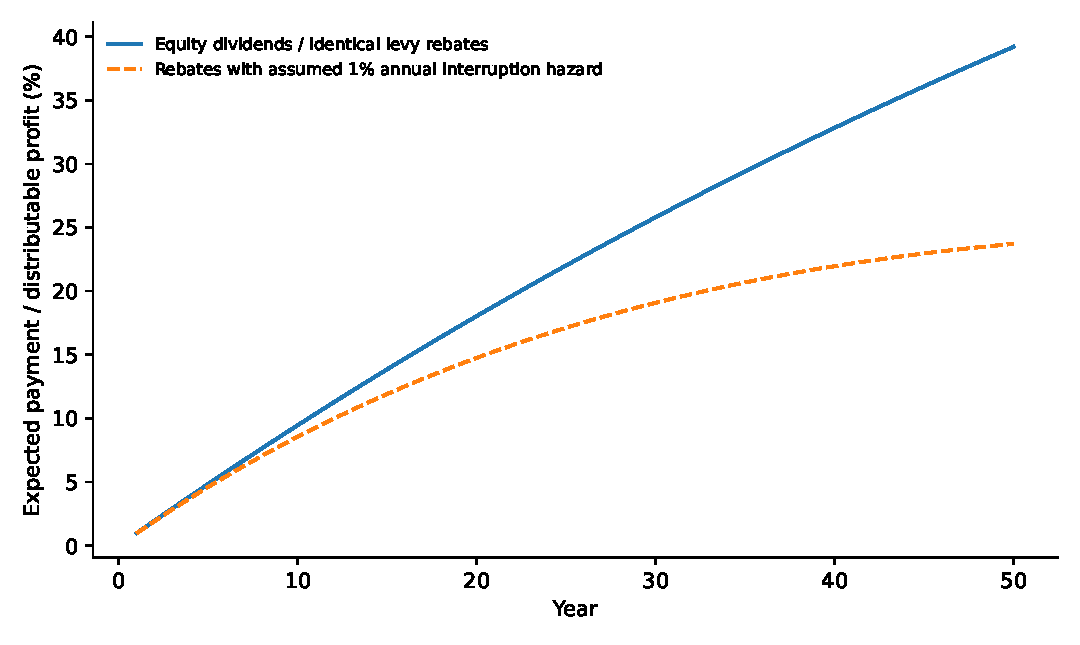
\includegraphics[width=.9\linewidth]{figures/conditional_durability.pdf}
\caption{A sensitivity illustration of the durability margin. The 1\% hazard is assumed, not measured. Equivalent hazards give equivalent expected payouts; the figure is not evidence that fiscal contracts are less secure.}
\end{figure}

\section{A closed heterogeneous-agent transition laboratory}
\subsection{Agents, production and resources}
There are $n_h=400$ equally weighted resident-equivalent agents and three representative firm types with output weights $\omega=(0.35,0.35,0.30)$. These represent diversified activities, not observed individual companies. Initial real GDP and the price level equal one, initial capital is three units and initial money is 0.6 units. Wage and equity distributions are correlated but heterogeneous synthetic draws. No household survey was used to estimate them.

The common automation trajectory is a normalised logistic function beginning at zero. Firm automation scales it by $(1,0.9,0.8)$. Slow, medium and fast cases differ in midpoint, speed, saturation and productivity gain. Automation changes the wage share according to $\lambda_{j,t}=0.10+0.48(1-a_{j,t})$. Thus labour income becomes less important by assumption; complete elimination of work is not imposed. Heterogeneous task exposure alters within-firm wage allocations and is then normalised to the wage bill. The resulting labour-demand index is a proxy, not measured unemployment.

Planned investment shares are
\begin{equation}
\nu_{j,t}=\operatorname{clip}(0.22+0.025a_{j,t}-\chi\delta_{j,t},\,0.04,\,0.40),\quad\chi=0.60,
\end{equation}
subject to a positive distributable residual. Shares of gross output allocated to wages, retained-earnings investment and cash dividends sum to one. Investment is gross; replacement investment and depreciation are not counted as household cash income. Capital evolves as
\begin{equation}
K_{j,t+1}=(1-0.06)K_{j,t}+\omega_j\nu_{j,t}Y_t.
\end{equation}
The raw capacity index is
\begin{equation}
Y_t^{\rm raw}=\sum_j\omega_j(1+g_A)^t\exp(\gamma a_{j,t})
\left(\frac{K_{j,t}}{K_{j,0}}\right)^{\beta},\quad g_A=0.01,\ \beta=0.40.
\end{equation}
A separate resource envelope bounds potential output:
\begin{equation}
Y_t^*=\min\left\{Y_t^{\rm raw},\frac{R_0(1+g_R)^t}{1+\eta\bar a_t}\right\},\quad
R_0=1.30,\ g_R=0.035,\ \eta=0.15.
\end{equation}
This deliberately exposes a possible resource bottleneck rather than hiding it in an optimistic TFP process. A temporary supply shock multiplies capacity by a three-year recovery profile. The reported raw-capacity/resource-capacity ratio is a pressure proxy, not a market-clearing resource price.

\subsection{Household flows and endogenous transaction demand}
Let $r_{i,t}$ be a household's share of current wages and distributable profits. It combines the normalised wage allocation and both equity classes; $\sum_i r_{i,t}=1-\nu_t$, where $\nu_t=\sum_j\omega_j\nu_{j,t}$. Given flat conventional tax rate $\tau_t$, household disposable income is
\begin{equation}
h^{\rm disp}_{i,t}=(1-\tau_t)r_{i,t}N_t+h_{i,t}.
\end{equation}
The protected-balance levy is applied to opening money. In the progressive version, the marginal rate is zero below 0.12 times forecast mean annual income, $d_t/2$ above that exemption, and $d_t$ above forecast mean annual income. The upper-bracket charge is therefore incremental rather than a discontinuity on the entire balance. The top rate begins at 4\% and can rise with previous inflation, capped at 15\%. A flat-rate comparator and the original 33\% proposal are separate tests.

Consumption is a share of currently available cash plus income:
\begin{equation}
C_{i,t}=\alpha_{i,t}\{m_{i,t-1}-b_{i,t}+h^{\rm disp}_{i,t}\},\qquad
\alpha_{i,t}=\frac{1}{1+\kappa_{i,t}}.\label{eq:cons}
\end{equation}
The liquidity ratio $\kappa_{i,t}$ decreases exponentially with expected inflation relative to target, the effective holding levy and the return advantage of alternatives. Its elasticity is four in the central scenario. Expectations adjust at rate 0.3. This is an explicit behavioural money-demand mechanism; it is not a fully optimising household portfolio model. In particular, a desire to escape money changes spending and prices, while the model has no offshore asset stock.

Money holdings satisfy
\begin{equation}
m_{i,t}=m_{i,t-1}-b_{i,t}+h^{\rm disp}_{i,t}-C_{i,t}.
\end{equation}
Here lower-case $m_i$ denotes an individual's \emph{nominal} account balance; only the aggregate $m=M/P$ in \eqref{M-eq:seign} denotes real balances. The code uses unambiguous `cash' and `real\_cash' names. The distinction prevents a nominal/real bookkeeping error.

\subsection{Nominal expenditure, output and prices}
Public purchases are 22\% of forecast nominal capacity. Transfers use \eqref{M-eq:floor}, evaluated on predicted after-tax factor income. The main floor is 25\% of forecast real GDP per resident-equivalent unit, indexed to potential output; it is not the transfer amount itself. A targeted comparator tops up individual predicted incomes, whereas the universal policy pays everyone the same amount required for the chosen tenth percentile.

Conditional on a tax rate, all nominal expenditure is solved jointly:
\begin{equation}
N_t=\frac{\sum_i\alpha_{i,t}(m_{i,t-1}-b_{i,t}+h_{i,t})+G_t}
{1-\nu_t-\sum_i\alpha_{i,t}(1-\tau_t)r_{i,t}}.\label{eq:nominal}
\end{equation}
The denominator must be strictly positive. This is an algebraic solution of the within-period goods and cash-flow equations, not an independently estimated expenditure multiplier. The price/output closure is
\begin{equation}
P_t=\max\left\{\frac{N_t}{Y_t^*},\,(1-\zeta)P_{t-1}\right\},\quad
Y_t=N_t/P_t,\quad\zeta=0.02.\label{eq:prices}
\end{equation}
Nominal demand above capacity raises prices; demand below the downward-adjustment limit lowers utilisation. Prices can fall by at most 2\% annually under this closure. Sectoral relative prices, wage bargaining, expectations-driven Phillips dynamics and optimal monetary policy are not estimated. Those omissions restrict external inference from the inflation paths.

\subsection{Policy rules and explicit fiscal closure}
The adaptive monetary rule targets a change in money informed by forecast capacity growth, average desired liquidity and the inflation gap:
\begin{equation}
\mu_t^*=\operatorname{clip}\left[(1+\pi^*)\frac{\widehat Y_t}{Y_{t-1}}
\frac{\bar\kappa_t}{\bar\kappa_{t-1}}-1+\psi(\pi^*-\pi_{t-1}),\,-0.15,\,0.20\right],
\end{equation}
with $\pi^*=2\%$ and $\psi=0.25$. It does not directly set current inflation. A scalar root solve selects $\tau_t\in[0,0.85]$ to attain $M_t=M_{t-1}(1+\mu_t^*)$ subject to the preceding flow equations. If no root is available, the closest boundary is used and a fiscal-capacity flag is recorded. In the fixed-money-growth case, the desired growth is 4\%. In fiscal-dominant cases, the conventional tax rate is fixed at 30\% of cash factor income, or at zero in the no-tax stress, and issuance adjusts residually to finance the budget.

This distinction is essential to interpretation. A path near the inflation target in the adaptive model can be enabled by high residual taxation. It is not a demonstration that programmable money or demurrage autonomously finances expenditure. Likewise, the maximum tax bound is a design parameter, not a claim that a society could immediately implement an 85\% tax rate. The fiscal-capacity stress reduces that bound to 35\%.

\subsection{Balance sheets and validation}
Household assets are sovereign money plus firm book equity. Firms hold productive capital and issue matching equity claims. The consolidated government is the issuer of money with negative financial net worth equal to outstanding money in this simplified model. Aggregate private and public financial claims net to zero; real national wealth is capital. Public infrastructure, foreign wealth and government debt are excluded, not silently assigned zero empirical values.

\begin{table}[htbp]\centering\small
\caption{Model balance-sheet accounting at book value}
\begin{tabular}{@{}lrrrr@{}}
\toprule
Item & Households & Firms & Government & Total\\
\midrule
Sovereign money & $M$ & 0 & $-M$ & 0\\
Corporate equity & $PK$ & $-PK$ & 0 & 0\\
Productive capital & 0 & $PK$ & 0 & $PK$\\
Net worth & $M+PK$ & 0 & $-M$ & $PK$\\
\bottomrule
\end{tabular}
\end{table}

Every period checks $N=C+J+G$, $\Delta M=G+H-T-B$, non-negative cash and equity shares summing to one. The unit suite also tests dilution recursions, vesting, cash-settled secondary sales, exclusion, endogeneity of money demand, the analytical envelope, invalid inputs and deterministic reproduction. These checks establish implementation consistency, not the empirical truth of behavioural rules.


\section{Data anchors, scenarios and evaluation}
\subsection{Empirical anchors versus assumptions}
The European anchor is the 22 April 2026 first annual EDP notification for 2025. EU27 GDP is EUR18.826635 trillion, public expenditure 49.5\% of GDP and public revenue 46.4\%; the separate EA20 GDP is EUR15.838206 trillion \citep{eurostat2026}. A rounded 452 million EU resident count on 1 January 2026 provides an illustrative unit conversion \citep{population2026}. The two date conventions are disclosed. This is not an official GDP-per-capita series and not an adult population estimate. All per-person monetary illustrations are \emph{resident-equivalent} amounts; an adult-only programme requires a separate demographic calibration.

The model's 22\% public-purchases parameter is an assumed block of services, not the full 49.5\% general-government spending aggregate. Transfers are modelled separately. The latent automation coefficient is not inferred from the current proportion of firms using an AI tool. Neither the money/GDP ratio nor the contribution distribution is estimated from present EU data. In particular, a euro-area M3 numerator is not divided by an EU27 denominator. An attempted direct API retrieval was unavailable in the execution environment; the package instead supplies explicit manually transcribed official anchors with URLs and a separate optional refresh script.

\begin{table}[htbp]\centering\small
\caption{Principal central parameters: all behavioural entries are scenario assumptions}
\begin{tabularx}{\linewidth}{@{}p{.34\linewidth}p{.18\linewidth}X@{}}
\toprule
Quantity & Central value & Interpretation\\
\midrule
Population and firm types & 400; 3 & Synthetic equal-weight agents and representative activities\\
Initial capital/output; money/output & 3.0; 0.60 & Post-reform starting stocks, not observed EU aggregates\\
Trend productivity; depreciation & 1\%; 6\% & Annual production parameters\\
Capital elasticity & 0.40 & Reduced-form capacity elasticity\\
Income reference floor & 25\% & Share of potential GDP per resident equivalent\\
Public purchases & 22\% & Separate assumed public-service block\\
Annual equity issue cap & 2\% & Relative to old share count, conditional on automation\\
Automation threshold & 0.25 & Start of participant-share issuance\\
Top levy; protected balance & 4\%; 0.12 & Initial top rate; exemption in forecast mean-income units\\
Liquidity-cost elasticity & 4 & Unestimated behavioural response\\
Resource growth & 3.5\% & Stylised annual capacity constraint\\
Investment response to dilution & 0.60 & Sensitivity parameter, not an identified elasticity\\
\bottomrule
\end{tabularx}
\end{table}

\subsection{Counterfactuals and uncertainty design}
The ten policy cases share the same accounting. B0 is a targeted tax-transfer comparator, not a fitted present-day EU system. B1 supplies no household transfer. B2 combines a universal top-up with the adaptive monetary rule and residual taxes; it is a conventional tax-adjusted benchmark with ordinary monetary accommodation, not literally zero seigniorage. B3 fixes the tax rate and lets money finance transfers. B4 adds demurrage to B3. B5 adds usownership to B2 without the special levy. B6 is the hybrid with usownership, adaptive money and progressive levy. B7 substitutes equal firm-specific citizen grants as a coverage comparator. B8 uses fixed money growth with usownership and the levy. B9 imposes zero conventional tax. Neither B7 nor the hundred-year paths forces pooled ownership.

Slow automation has logistic midpoint 40, speed 0.08, saturation 0.65 and productivity gain 0.35. Medium uses 20, 0.14, 0.90 and 0.90; fast uses 10, 0.30, 0.98 and 1.60. These define paths rather than probabilities. The three paths across ten policies generate 30 main simulations. Outputs are reported at years 10, 25, 50 and 100 when the numerical path remains admissible. Runs crossing a very high price-level or inflation threshold are stopped and future observations remain missing, not extrapolated or filled with zeros.

Thirty-six additional experiments vary the floor, indexation, levy, monetary demand, fiscal capacity, resource capacity, investment response, exclusion, score capture and share transferability. A Latin-hypercube design varies ten parameters over stated intervals for 128 common configurations and runs B2, B5 and B6 on each. The 384 outcomes use the same household draws within a configuration; common random numbers improve comparability. These draws are exploration of a chosen parameter box, not a posterior distribution or probability of real-world success.

Success is multidimensional. We report inflation, output, fiscal needs, monetary balances, median income, wealth concentration and coverage shortfalls. A narrow \emph{transfer-sunset} flag requires MVI below 1\% of GDP for the final five years of the fifty-year window; it is not the same as universal adequacy. A price-band flag requires absolute annual inflation no higher than 5\% throughout the path. Log consumption is a diagnostic and is not used to claim welfare optimality in the absence of leisure, risk and public-service utility.


\section{Results}
\subsection{The monetary bridge remains fiscally constrained}
Table~\ref{tab:bench} gives the medium-path year-50 comparisons. In B6, MVI is \ResultPSixMviGdp\% of GDP compared with \ResultPTwoMviGdp\% under B2. Conventional tax revenue nevertheless remains \ResultPSixTaxGdp\% of GDP. The hybrid is not a tax-free equilibrium. The baseline path has a small opening monetary contraction while balances and the levy adjust; negative issuance is retained in the data rather than relabelled as positive seigniorage.

\begin{table}[htbp]\centering\small
\caption{Medium automation at year 50; peak inflation covers the entire available path}\label{tab:bench}
\begin{tabular}{lllllll}
\toprule
Policy & Complete & Real GDP & MVI/GDP & Tax/GDP & Wealth Gini & Peak inflation \\
\midrule
B0 & yes & 6.48 & 7.1\% & 25.0\% & 0.768 & 2.1\% \\
B1 & yes & 6.48 & 0.0\% & 17.8\% & 0.788 & 2.0\% \\
B2 & yes & 6.48 & 19.0\% & 37.0\% & 0.754 & 2.2\% \\
B3 & yes & 6.48 & 12.4\% & 22.8\% & 0.800 & 40.3\% \\
B4 & yes & 6.48 & 12.0\% & 22.8\% & 0.804 & 45.1\% \\
B5 & yes & 6.48 & 10.6\% & 28.5\% & 0.583 & 2.1\% \\
B6 & yes & 6.48 & 10.2\% & 27.1\% & 0.584 & 2.1\% \\
B7 & yes & 6.48 & 6.0\% & 23.9\% & 0.560 & 2.1\% \\
B8 & yes & 6.46 & 11.0\% & 29.0\% & 0.578 & 8.6\% \\
B9 & no & -- & -- & -- & -- & -- \\
\bottomrule
\end{tabular}

\par\smallskip\footnotesize Real GDP is indexed to one initially. Missing year-50 values indicate a stopped numerical path. B9's extreme peak is a model-breakdown diagnostic, not a quantitative inflation forecast.
\end{table}

Fiscal dominance produces a materially different result. With the fixed 30\% factor-income tax, B3 reaches roughly 40.3\% peak annual inflation. Adding the holding levy in B4 raises the peak to roughly 45.1\% in this configuration. The consumption-liquidity response can offset or reverse the mechanical contraction from the fee. These are model-specific counterexamples to a guarantee that demurrage stabilises prices. They do not establish that every negative-rate policy is inflationary.

The central no-tax B9 run crosses the numerical inflation guard after five years in the medium path, before meaningful automation-linked ownership has accumulated. The exact extreme rate has no predictive interpretation; it demonstrates failure of this closure under the combination of public purchases, transfer promises and collapsing demand for balances. Lower MVI/GDP during that episode is partly erosion of real transfers, not successful replacement by capital income. A separate narrow-state test reduces public purchases to the source proposal's 7\% of forecast output. With a lower income floor of 15\% and initial money/GDP of one, the no-tax path remains numerically admissible for fifty years and eventually eliminates the top-up, although peak inflation exceeds 7\%. At initial money/GDP of 0.6, closely related narrow-state cases fail. This is a conditional survival case, not evidence of unchanged public services or of a 2\% inflation regime. It illustrates why money demand and the service/floor commitment must be tested jointly. Conversely, adaptive cases remain near 2\% only because taxation adjusts. Most of the reduced transfer burden in B6 is reflected in lower tax requirements, not in an independently identified monetary-finance dividend.

\begin{figure}[htbp]\centering
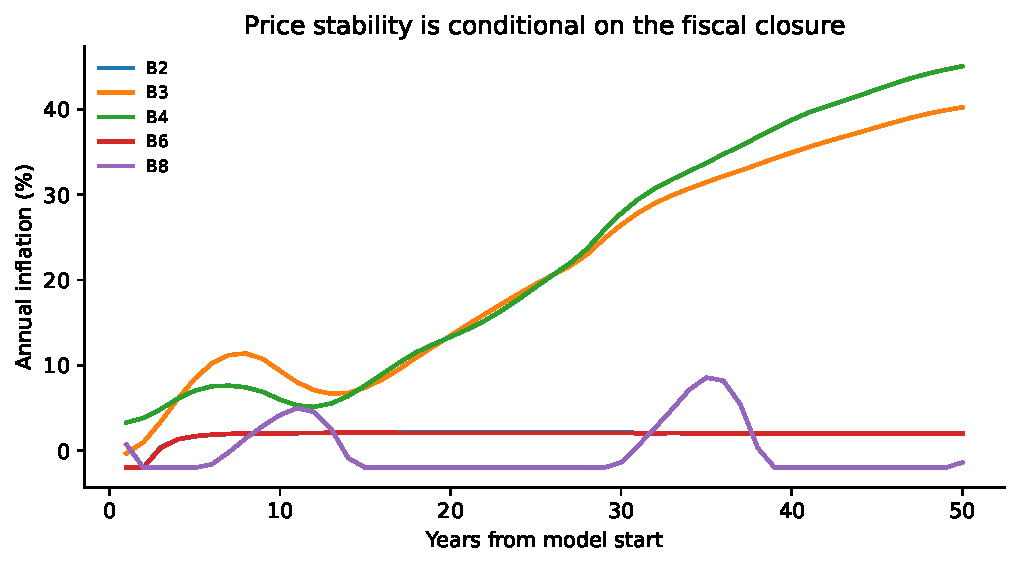
\includegraphics[width=.92\linewidth]{figures/inflation_paths.pdf}
\caption{Inflation under alternative fiscal--monetary closures. A near-target hybrid path is conditional on residual taxation and the stipulated price mechanism.}
\end{figure}
\begin{figure}[htbp]\centering
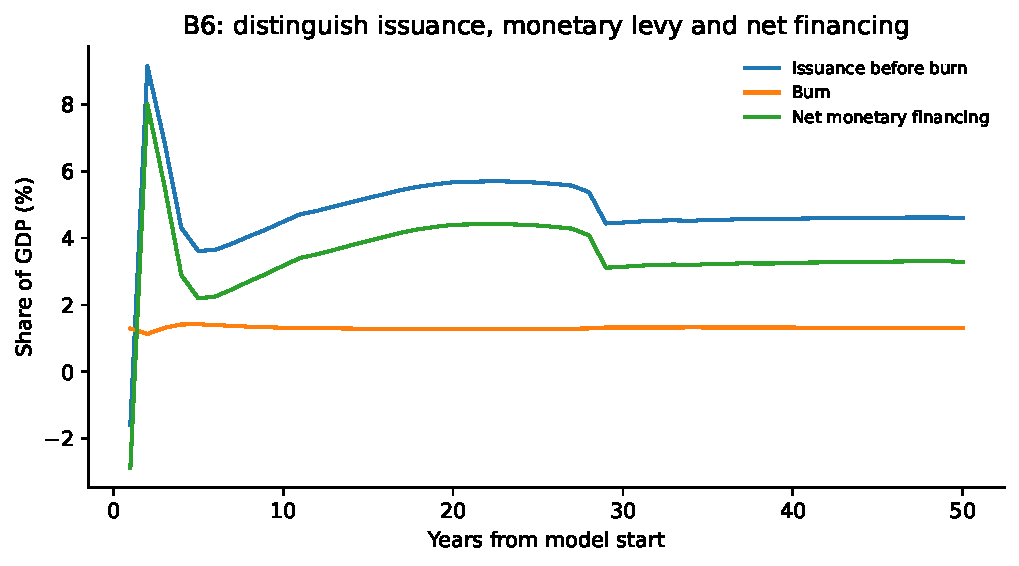
\includegraphics[width=.92\linewidth]{figures/monetary_flows.pdf}
\caption{Hybrid monetary flows. The difference between issuance before burn and net monetary financing is the holding levy. These flows are not additive independent sources of free resources.}
\end{figure}

\subsection{Ownership diffusion and distribution}
User equity reaches \ResultPSixUsownershipShare\% by year 50 in the medium path. The wealth Gini is \ResultPSixGiniWealth, against \ResultPTwoGiniWealth\ in B2 and \ResultPOneGiniWealth\ in the no-transfer comparator. The relevant wealth measure is real transaction balances plus book-valued corporate equity, not an estimate of total EU household wealth. The central synthetic initial distribution is highly concentrated, so the absolute Gini levels should not be read as calibrated observations.

The B5/B6 comparison isolates much of the levy increment. Without special demurrage, B5 reaches a wealth Gini of \ResultPFiveGiniWealth\ and MVI of \ResultPFiveMviGdp\% of GDP. B6's extra levy lowers the conventional tax requirement, but its wealth Gini is slightly higher. Thus this experiment attributes most of the ownership effect to equity diffusion, not to programmable monetary decay. Equal firm-specific grants in B7 achieve a lower Gini and smaller transfer requirement than contribution weighting, at the cost of dropping the proposed link between individual participation and grants. That is an objective trade-off, not a reason to silently redefine usownership.

\begin{figure}[htbp]\centering
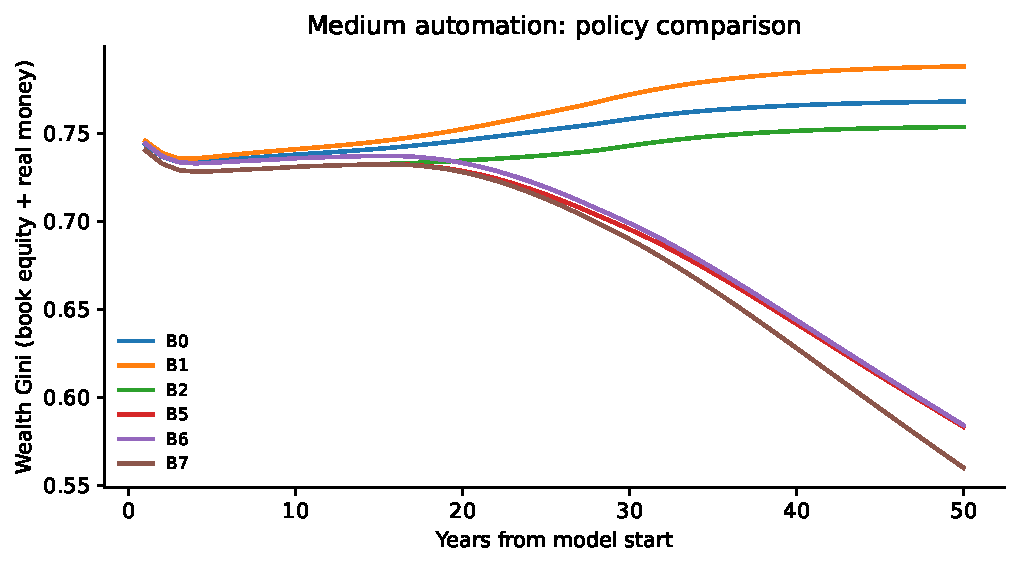
\includegraphics[width=.92\linewidth]{figures/wealth_paths.pdf}
\caption{Wealth distribution in the medium path. Levels depend on the synthetic starting distribution; comparisons hold the accounting and initial draws fixed.}
\end{figure}
\begin{figure}[htbp]\centering
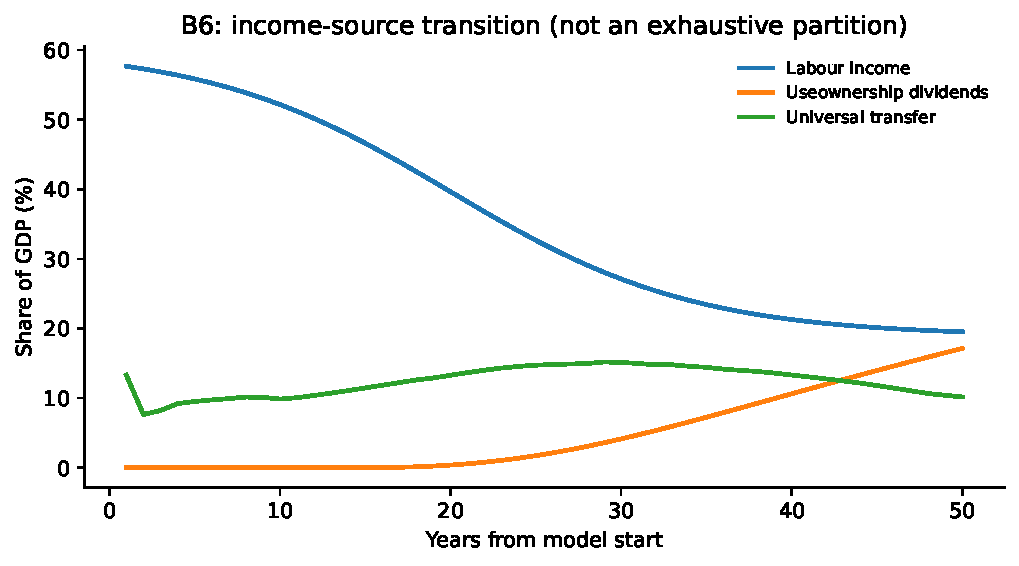
\includegraphics[width=.92\linewidth]{figures/income_transition.pdf}
\caption{The hybrid's income-source transition. Labour, user dividends and transfers are shown separately; ordinary dividends and taxes mean these curves are not an exhaustive GDP partition.}
\end{figure}

\subsection{The transfer peak and the conditional sunset}
The medium B6 path's transfer/GDP ratio peaks at approximately 15.19\% in model year 29, then falls to 10.16\% at year 50. It drops below 1\% around year 82 in the extension and reaches zero by year 100. Slow automation still requires about 8.02\% of GDP at year 100. Fast automation attains greater user ownership and a zero quantile-based transfer by that horizon. These are conditional trajectories under unchanged institutions and synthetic cohorts, not dated forecasts of Europe.

The main pattern does support a gradual ownership bridge, but not an automatic rapid one. A 2\% annual maximum issue is much slower than an immediate ownership redistribution, particularly because the threshold delays issuance. Grant recipients also continue to be heterogeneous. The time at which an aggregate transfer becomes small depends on the floor, payout share, tax incidence and lower-tail participation, not just the aggregate value of automated capital.

\begin{table}[htbp]\centering\small
\caption{Hybrid scenario horizons: no compulsory pooling at any horizon}
\begin{tabular}{lllllll}
\toprule
AI path & Year & Real GDP & User equity & MVI/GDP & Tax/GDP & Wealth Gini \\
\midrule
slow & 10 & 1.18 & 0.0\% & 9.4\% & 27.5\% & 0.737 \\
slow & 25 & 1.56 & 0.0\% & 10.1\% & 27.8\% & 0.740 \\
slow & 50 & 2.72 & 2.8\% & 13.7\% & 31.3\% & 0.731 \\
slow & 100 & 7.25 & 33.2\% & 8.0\% & 26.0\% & 0.559 \\
medium & 10 & 1.31 & 0.0\% & 9.9\% & 26.9\% & 0.736 \\
medium & 25 & 2.69 & 3.9\% & 14.7\% & 30.6\% & 0.719 \\
medium & 50 & 6.48 & 29.7\% & 10.2\% & 27.1\% & 0.584 \\
medium & 100 & 17.67 & 66.3\% & 0.0\% & 18.1\% & 0.371 \\
fast & 10 & 1.72 & 0.8\% & 14.4\% & 32.2\% & 0.733 \\
fast & 25 & 2.72 & 19.0\% & 14.3\% & 31.3\% & 0.648 \\
fast & 50 & 6.41 & 46.6\% & 4.7\% & 21.6\% & 0.490 \\
fast & 100 & 35.79 & 76.7\% & 0.0\% & 17.2\% & 0.311 \\
\bottomrule
\end{tabular}

\par\smallskip\footnotesize Years are elapsed model years. Output multipliers over 100 years are scenario arithmetic, not forecasts. Demography, firm turnover and new generations are not included.
\end{table}

A fixed-real-floor experiment produces an earlier sunset than the prosperity-indexed floor. A lower relative floor of 15\% also reaches a negligible transfer within the fifty-year window, whereas a 40\% relative floor leaves about 30.63\% of GDP in transfers at year 50. These differences are economically substantive. A policy that protects only an initial subsistence basket is not equivalent to a policy allowing displaced households to share proportionately in AI-driven prosperity.

\begin{figure}[htbp]\centering
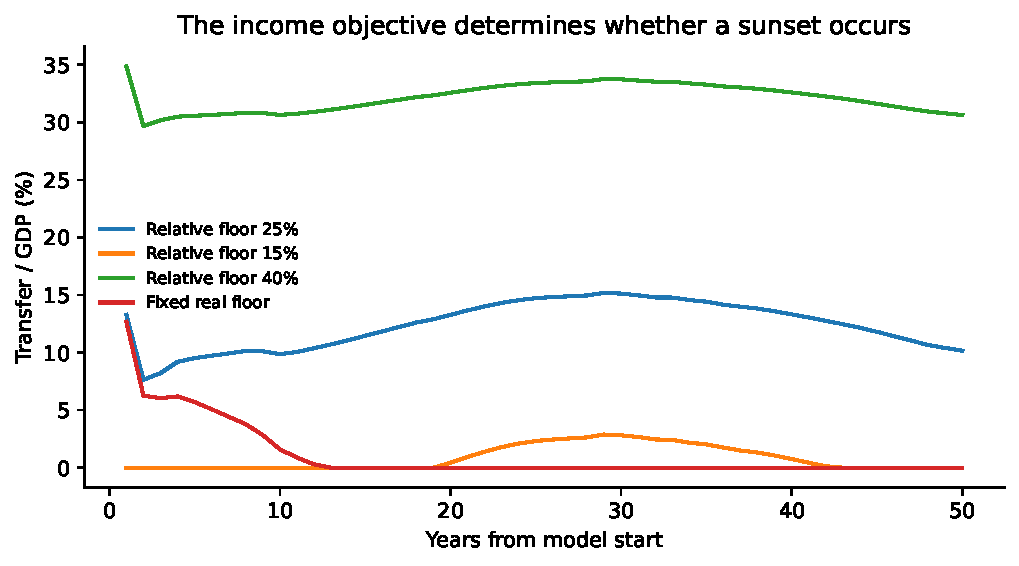
\includegraphics[width=.92\linewidth]{figures/sunset_conditions.pdf}
\caption{Different income objectives give different sunset conclusions. A shrinking transfer ratio is not alone evidence of equitable participation in abundance.}
\end{figure}

\subsection{Coverage, manipulation and reconcentration}
Excluding the lowest-initial-wage 20\% of synthetic participants from equity grants leaves aggregate user equity unchanged but raises year-50 MVI to about 19.15\% of GDP, nearly the B2 no-usownership requirement. This illustrates the coverage condition in the main paper: total ownership diffusion and adequate coverage are distinct. The low contributors still receive the separate universal transfer; the experiment does not endorse conditioning their basic support on participation.

Consumption-only allocation produces a year-50 wealth Gini near 0.660 rather than 0.584. Giving a synthetic attacker 20\% of score mass raises it to about 0.624. Such score capture is not a forecast of a specific bot exploit; it is a stress on measurement integrity. More sophisticated contribution scoring is therefore not automatically more equitable or harder to manipulate than a simple rule.

With immediate permitted liquidation, simulated user equity falls to about 7.72\% and the wealth Gini rises to about 0.753. Ten-year vesting with a 20\% retained core moderates this effect: user equity is about 19.11\% and the Gini about 0.663. These findings are conditional on cash-constrained wealthy buyers and book-value pricing. They identify a reconcentration channel but do not estimate the value of actual legal restrictions or the optimal vesting period.

\begin{figure}[htbp]\centering
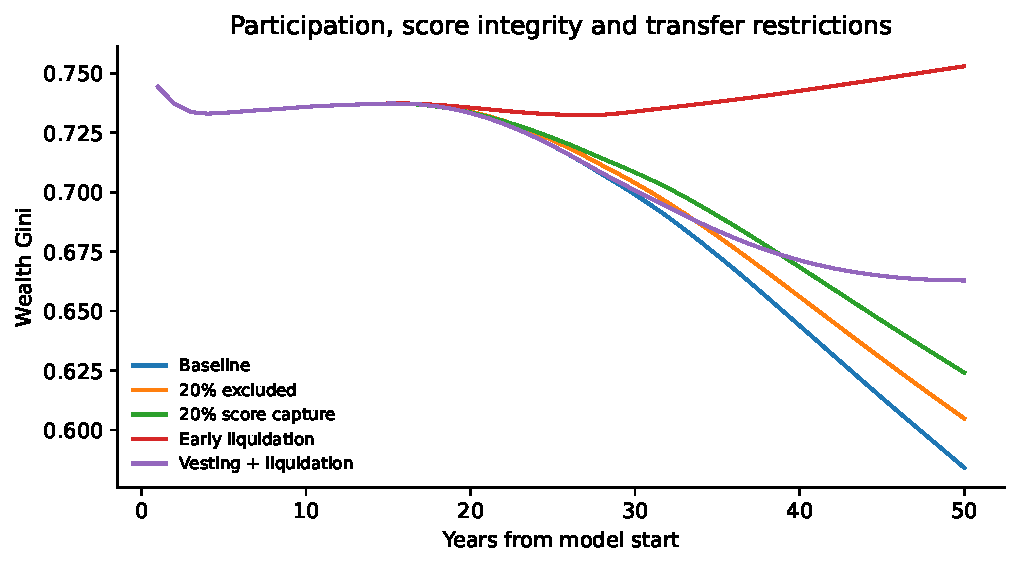
\includegraphics[width=.92\linewidth]{figures/participation_risks.pdf}
\caption{Distributional risks from exclusion, score capture and secondary liquidation. The baseline's retained user shares are a substantive institutional assumption.}
\end{figure}

\subsection{Resource and investment trade-offs}
The central resource constraint binds sufficiently strongly that several policies share the same year-50 real-output level. That equality is not a finding that ownership has no productivity cost; it is partly a property of the binding ceiling. Removing that binding ceiling exposes the assumed investment penalty. At year 50, real GDP is approximately 6.862 with zero dilution penalty, 6.738 with the central penalty and 6.227 with the high penalty. Increasing the penalty can raise current distributable profits by reducing retained investment and can therefore reduce MVI even while long-run output deteriorates. Judging success solely by a smaller transfer bill would reward that undesirable outcome.

The resource envelope also explains why the fast-automation path need not dominate medium automation at every finite date. Greater automation can tighten the assumed resource intensity constraint before later capital/productivity growth changes which constraint binds. No ranking of real-world AI development speeds follows from that particular functional form. The point is to make non-monotonicity and bottlenecks visible rather than to guarantee abundance by construction.

\begin{figure}[htbp]\centering
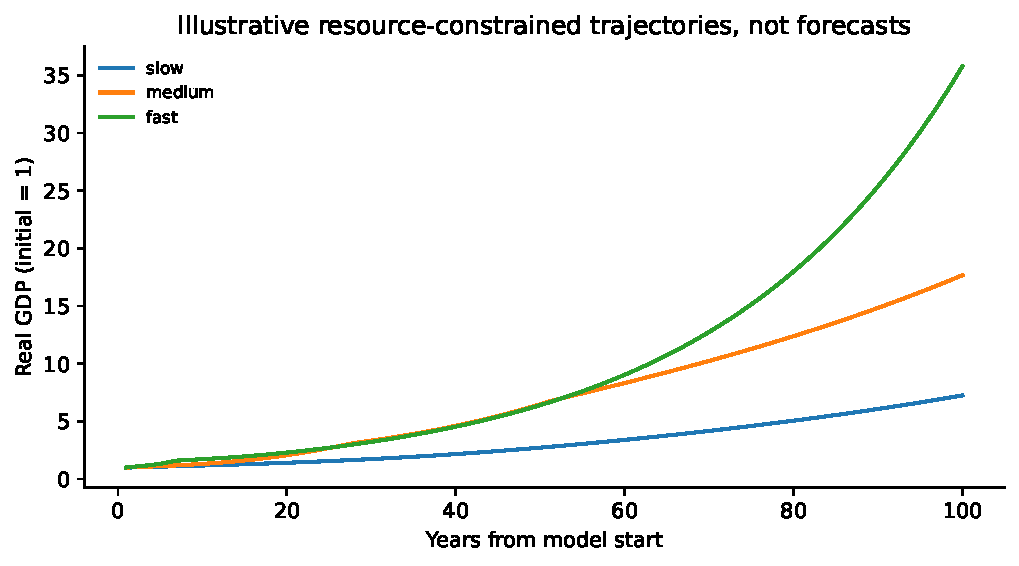
\includegraphics[width=.92\linewidth]{figures/real_output.pdf}
\caption{Resource-constrained scenario trajectories. A century-scale multiplier depends on compounded assumptions and should not be described as a forecast.}
\end{figure}


\section{Robustness, falsification and interpretation}
\begin{table}[htbp]\centering\small
\caption{Selected fifty-year hybrid robustness experiments}
\begin{tabular}{lllll}
\toprule
Experiment & MVI/GDP & Wealth Gini & Tax/GDP & Peak inflation \\
\midrule
baseline & 10.2\% & 0.584 & 27.1\% & 2.1\% \\
low relative floor & 0.0\% & 0.604 & 16.7\% & 2.1\% \\
high relative floor & 30.6\% & 0.549 & 48.0\% & 2.1\% \\
fixed real floor & 0.0\% & 0.605 & 16.7\% & 2.1\% \\
historical 33pct levy & 9.1\% & 0.589 & 23.4\% & 34.4\% \\
supply shock & 10.2\% & 0.584 & 27.1\% & 27.7\% \\
fiscal capacity limit & 10.0\% & 0.585 & 26.5\% & 9.5\% \\
low coverage & 19.1\% & 0.605 & 36.2\% & 2.1\% \\
score attack & 12.3\% & 0.624 & 29.3\% & 2.1\% \\
consumption scores & 14.3\% & 0.660 & 31.3\% & 2.1\% \\
equal grants comparator & 5.4\% & 0.560 & 22.3\% & 2.1\% \\
liquidation no vesting & 18.2\% & 0.753 & 35.2\% & 2.1\% \\
liquidation with vesting & 14.3\% & 0.663 & 31.3\% & 2.1\% \\
\bottomrule
\end{tabular}

\end{table}

An unanticipated 20\% supply disruption produces peak inflation around 27.66\% despite the adaptive rule. A 40\% liquidity-preference shock produces about 25.69\%. Optimistic output forecasting, a restrictive fiscal-capacity ceiling and the 33\% levy also break the narrow central price pattern. A feedback architecture must therefore be evaluated with forecast error and bounded instruments; deterministic target tracking is not robustness.

In the 128 paired parameter designs, B6 lowers the wealth Gini relative to B2 in all configurations. The median reduction is about 0.169 Gini units in this particular synthetic design. MVI/GDP is lower in 106 configurations and conventional tax/GDP in 124. Output is lower in 61, with the remaining cases generally limited by a common resource ceiling. Only six hybrid configurations meet the final-five-year MVI-below-1\% criterion, compared with four under B5 and none under B2. All 128 adaptive hybrid configurations remain within the defined 5\% annual price band, but the parameter box does not include the discrete supply and money-demand shocks that generate large inflation in the separate stress tests. These frequencies are not estimated probabilities of policy success.

\begin{figure}[htbp]\centering
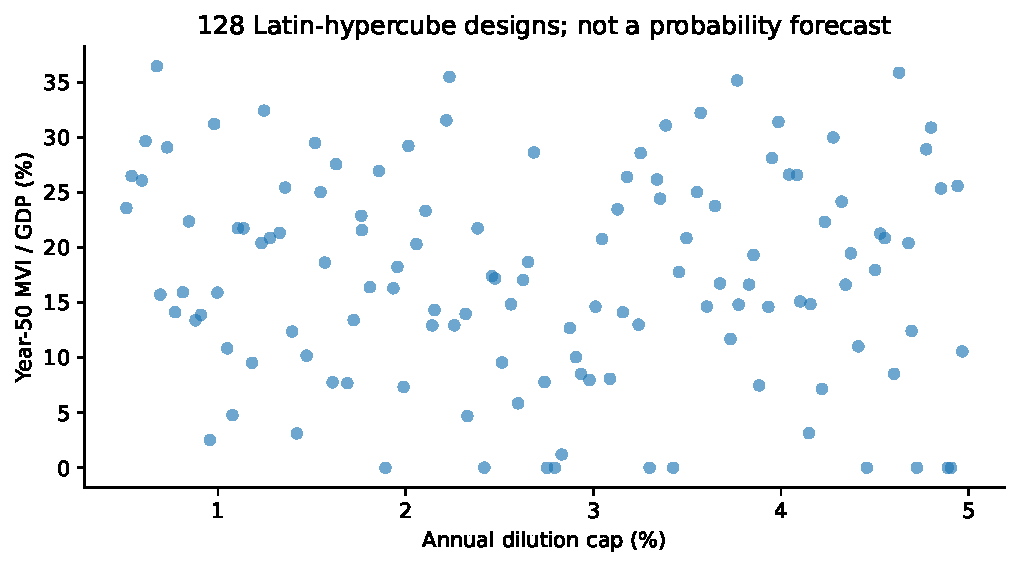
\includegraphics[width=.92\linewidth]{figures/sensitivity_scatter.pdf}
\caption{The transfer outcome depends on more than the dilution cap. The plotted Latin-hypercube box is exploratory, not a distribution of forecast uncertainty.}
\end{figure}

The results support a narrower set of hypotheses than the motivating proposal. Firm-specific equity can improve dispersion under the assumed grant rules, and enough broadly received capital income can replace a specified income top-up. The tests reject a universal claim that demurrage stabilises prices, an unconditional sunset, and the adequacy of aggregate ownership statistics as evidence of lower-tail coverage. They do not establish that a seigniorage-led bridge dominates a conventional tax-financed transition. In the successful monetary cases, flexible fiscal support is doing substantial stabilising work.

This separation also prevents a circular interpretation of the policy rule. If the government changes taxes until a desired money path is attained, low inflation is partly a consequence of the combined fiscal--monetary design. It cannot be cited as evidence that taxes were unnecessary. The relevant research question becomes how much of the transitional fiscal need can be safely allocated to monetary financing, given independent estimates of money demand and available fiscal capacity.


\section{Comparative extension: implementation and robustness}
The additional policies are defined in \texttt{scripts/run\_comparisons.py}. B10 applies labour and capital tax multipliers 0.6 and 1.4, with each effective rate capped at 0.95. Transfers are recomputed from the net-income vector during the fiscal root solve, rather than incorrectly applying a scalar factor to a pre-tax quantile. B11 and B12 use the shadow-register pass-through described above; B13 uses targeted predicted-gap protection with the hybrid. The code preserves the inherited default policy rules to numerical tolerance.

The 27 new main comparison runs use nine policies over three automation paths for 50 years. The 72 additional robustness runs use B0, B2, B5, B6, B10 and B13 under twelve common settings: central; investment penalty 3; no investment penalty; 20\% contributor exclusion; 4\% annual issue cap; 0.5\% cap; 7\% public purchases; 30\% public purchases; fixed-real floor; liquidity elasticity 10; 20\% score capture; and resource growth 1.2\%. Unmentioned parameters retain the baseline. These are selected sensitivities, not a posterior or global optimal-policy search.

The contribution register is fictional in the simulation. The user fractions are conserved exactly but the scoring weights are not estimated economic values. The same initial household draws, production opportunities, resource limits and services are used within each comparison. The matched-levy tests use the same investment penalty as equity by construction; separately estimated responses could break the equivalence of realised outcomes.

\section{Reproduction and verification}
Run \texttt{python scripts/reproduce\_all.py --compile} from the repository root after installing its pinned dependencies. The pipeline regenerates the 450 inherited macro paths, all 99 comparative paths, analytical tables and figures. It then compiles the main manuscript and this supplement when LaTeX is installed. The exact command, environment and configuration are included in the repository. No access to the private exploratory notebooks is needed for the published numerical results.

The test suite checks monetary and goods accounting, legal and shadow equity conservation, nonnegative holdings, identical matched cash outcomes, invalid input rejection, deterministic results, generated table consistency and legacy-regression values. Tests cannot validate the external realism of an assumed behavioural equation. The largest baseline-accounting discrepancies are at floating-point precision. Full configurations and CSV outputs are supplied, including failed paths rather than replacing them with extrapolations.

\bibliographystyle{plainnat}\bibliography{bibliography}
\end{document}
